\chapter{Estudo Experimental de Software}

Este capítulo provê o roteiro de experimentação de software para ferramentas de ETL utilizando dados estruturados, semi estruturados e não estruturados. A Engenharia de Software Experimental tem como objetivo aprimorar métodos, técnicas e ferramentas de Engenharia de Software a partir de métodos experimentais (\cite{souza:2015}). As etapas definidas no processo de experimentação em Engenharia de Software proposto por \cite{souza:2015} consiste em etapas de definição, planejamento, operação, interpretação dos dados e empacotamento que serão melhor detalhados nas seções a seguir.
\clearpage

\section{Objetivos do experimento}

O objetivo principal da aplicação deste experimento é definir se o framework proposto por esta pesquisa de dissertação é uma ferramenta adequada para auxiliar no desenvolvimento de processos de ETL em dados estruturados, semi estruturados e não estruturados.

\subsection{Objetivo da Medição}

Tendo como base as ferramentas de ETL existentes na literatura, caracterizar:

\begin{enumerate}
	\item Quais as principais funcionalidades que as ferramentas de ETL oferecem:
	\begin{enumerate}
		\item essas funcionalidades manipulam dados estruturados, semi estruturados e não estruturados.
		\item  essas funcionalidades não manipulam dados estruturados, semi estruturados e não estruturados.
	\end{enumerate}
	\item Quais funcionalidades podem ser consideradas fundamentais para a produtividade na criação de processos de ETL:
	\begin{enumerate}
		\item quais necessitam manipular dados em grande escala.
		\item quais não manipulam grande volume de dados.
	\end{enumerate}
	\item Quais funcionalidades poderiam aprimorar as ferramentas de ETL.
\end{enumerate}

\subsection{Objetivos do Estudo}

\begin{itemize}
	\item Analisar as ferramentas de ETL para dados estruturados, semi estruturados e não estruturados;
	
	\item Com o propósito de caracterizar;
	
	\item Com respeito à intersecção das ferramentas de ETL existente;
	
	\item Do ponto de vista da literatura;
	
	\item No contexto comparativo entre as ferramentas mais conhecidas no mercado atual.
\end{itemize}


\subsection{Questões}

\begin{itemize}
	\item[Q1.] Existem funcionalidades listadas pelas ferramentas pesquisadas que não estão presentes no ETL4NoSQL?

	Métrica: A lista de funcionalidades que não estão presentes no ETL4NoSQL.

	\item[Q2.] Existem funcionalidades listadas pelas ferramentas pesquisadas que estão presentes no ETL4NoSQL, mas são consideradas pouco úteis?

	Métrica: A lista de funcionalidades que estão presentes nas ferramentas da literatura e no ETL4NoSQL e são consideradas inúteis.

	\item[Q3.] Existem funcionalidades que estão presentes nas ferramentas de ETL da literatura e no ETL4NoSQL, consideradas úteis, e que poderiam ser melhoradas?

	Métrica: A lista de funcionalidades que estão presentes nas ferramentas de ETL da literatura e no ETL4NoSQL, consideradas úteis e que necessitam melhorar.

	\item[Q4.] Existem funcionalidades que estão presentes nas ferramentas de ETL da literatura que não estão presentes no ETL4NoSQL, mas que são consideradas úteis?

	Métrica: A lista de funcionalidades que estão presentes nas ferramentas de ETL da literatura que não estão presentes no ETl4NoSQL e que são consideradas úteis.
\end{itemize}

\section{Planejamento}

Na etapa de planejamento são definidas as hipóteses do estudo, a descrição da instrumentação, as métricas, seleção do contexto e dos indivíduos, as variáveis, a análise qualitativa e a validade do experimento. Todas elas serão descritas nas seções seguintes.

\subsection{Definição das Hipóteses}

Hipótese nula (H0): As funcionalidades oferecidas pelo ETL4NoSQL são similares às funcionalidades oferecidas pelas ferramentas presentes na literatura.

Fp - Funcionalidades do ETL4NoSQL;

Fl - Funcionalidades das ferramentas da literatura.

H0: Fl - (Fp $\cap$ Fl) = $\emptyset$
\newline

Hipótese alternativa (H1): A lista de funcionalidades oferecidas pelo ETL4NoSQL é diferente da lista de funcionalidades oferecidas pelas ferramentas presentes na literatura.

Fp - Funcionalidades do ETL4NoSQL;

Fl - Funcionalidades das ferramentas da literatura.

H1: Fl - (Fp $\cap$ Fl) $\neq$ $\emptyset$
\newline

Hipótese alternativa (H2): Na lista de funcionalidades oferecidas pelo ETL4NoSQL e pelas ferramentas de ETL da literatura possuem funcionalidades consideradas pouco úteis.

Fpl - Funcionalidades presentes no ETL4NoSQL e nas ferramentas da literatura;

Fplu - Funcionalidades presentes no ETL4NoSQL e nas ferramentas da literatura que são consideradas úteis.

H2: Fpl - (Fpl $\cap$ Fplu) $\neq$ $\emptyset$
\newline


Hipótese alternativa (H3): Na lista de funcionalidades oferecidas pelo ETL4NoSQL e pelas ferramentas de ETL da literatura possuem funcionalidades consideradas úteis, cujo necessita de melhorias.

Fplu - Funcionalidades presentes no ETL4NoSQL e nas ferramentas da literatura que são consideradas úteis;

Fplun - Funcionalidades presentes no ETL4NoSQL e nas ferramentas da literatura que são consideradas úteis, cujo necessita melhorias.

H3: Fplu - (Fplu $\cap$ Fplun)  $\neq$ $\emptyset$
\newline

Hipótese alternativa (H4): A lista de funcionalidades que estão presentes nas ferramentas da literatura e não estão presentes no ETL4NoSQL que são consideradas úteis.

Fpn - Funcionalidades de ETL4NoSQL não presentes (Fpn $\equiv$  Fl - (Fp $\cap$ Fl))

Fo - Funcionalidades não presentes no ETL4NoSQL, mas que são consideradas úteis.

H4: Fpn - (Fpn $\cap$ Fo) $\neq$ $\emptyset$

\subsection{Descrição da instrumentação}

Para cada funcionalidade presente nas ferramentas apresentada na literatura que são consideradas fundamentais para o funcionamento dos processos de ETL pode ser encontrada no quadro \ref{instrumentacao}:

\begin{table}[ht]
	\centering
	\caption{Descrição da Instrumentação}
	\label{instrumentacao}
	\begin{tabular}{|p{5cm}| p{5cm} | p{5cm}|}
		\hline
		Presença da Funcionalidade (P) & Melhoria da Funcionalidade (M) & Utilidade da Funcionalidade (U)\\
		\hline
		\begin{enumerate}
			\item Não está presente
			\item Está presente parcialmente
			\item Está presente
		\end{enumerate} & 
		\begin{enumerate}
			\item Necessita melhorar
			\item Não há necessidade de melhoria
			\item Pode melhorar, mas não necessidade
		\end{enumerate} &
		\begin{enumerate}
			\item É útil
			\item Não é útil
			\item É parcialmente útil
		\end{enumerate}\\
		\hline
		
	\end{tabular}
\end{table}

Para cada funcionalidade aplicar teste estatístico qui-quadrado para definir:

se pode considerar que essa funcionalidade é fornecida;

se pode considerar que essa funcionalidade é útil;

se pode considerar que essa funcionalidade necessita de melhoria.

Resultado: N funcionalidades com valores (P; M; U) onde P - presença {0 - não presente; 1 - presente}; U - utilidade {0 - não é útil; 1 - é útil}; melhoria {0 - não necessita melhorar; 1 - necessita melhorar}.

\subsection{Métricas}

Na tabela \ref{metricas} são apresentadas as métricas utilizadas neste experimento.

\begin{table}[ht!]
	\centering
	\caption{Métricas}
	\label{metricas}
	\begin{tabular}{|p{0.5cm}| p{0.5cm} | p{0.5cm}| p{0.5cm}|p{9cm}|p{3cm}|}
		\hline
		N$\circ$ & P & M & U & Descrição da Funcionalidade & Questões\\
		\hline
		1 & 0 & 0 & 0 & Não está presente, não necessita melhorar, não é útil & Q1, Q4\\
		\hline
		2 & 0 & 0 & 1 & Não está presente, não necessita melhorar, é útil & Q1, Q4\\
		\hline
		3 & 0 & 1 & 0 & Não está presente, necessita melhorar, não é útil & N/A\\
		\hline
		4 & 0 & 1 & 1 & Não está presente, necessita melhorar, é útil & Q1, Q4\\
		\hline
		5 & 1 & 0 & 0 & Está presente, não necessita melhorar, não é útil & Q2\\
		\hline
		6 & 1 & 0 & 1 & Está presente, não necessita melhorar, é útil & Q3\\
		\hline
		7 & 1 & 1 & 0 & Está presente, necessita melhorar, não é útil & Q2\\
		\hline
		8 & 1 & 1 & 1 & Está presente, necessita melhorar, é útil & Q3\\
		\hline
		
		
		
	\end{tabular}
\end{table}	

\subsection{Seleção do contexto}

De acordo com Travassos (2002), o contexto pode ser caracterizado conforme quatro dimensões:

\begin{itemize}
	\item o processo: on-line / off-line;
	\item os participantes: ferramentas de ETL;
	\item realidade: o problema real / modelado;
	\item generalidade: específico / geral.
\end{itemize}

Nosso estudo supõe o processo off-line porque as ferramentas não estão sendo testadas durante todo o tempo da utilização, mas em certo instante. Os participantes são as ferramentas de ETL encontradas na literatura. O estudo é modelado porque as funcionalidades das ferramentas não são caracterizadas durante a resolução do problema real, mas utilizando parâmetros subjetivos (ex. presença, utilidade e necessidade). As funcionalidades do ETL4NoSQL são comparadas com as ferramentas presentes na literatura, então, o contexto possui o caráter específico.

\subsection{Seleção dos indivíduos}

Como participantes para o estudo propõe-se utilizar as ferramentas encontradas na literatura. Assume-se que esses indivíduos estão presente em diversos estudos realizados e avaliados no meio acadêmico.

Para a escolha das ferramentas utilizadas neste estudo foi levado em consideração a semelhança da finalidade do uso com a ferramenta proposta. Seria conveniente utilizar para o estudo ferramentas que tem o objetivo de auxiliar processos de ETL em diversas estruturas de dados. Dessa forma, a seleção baseou-se nas características das ferramentas.

\subsection{Variáveis}


Variável independente: A lista de funcionalidades das ferramentas encontradas na literatura.

Variáveis dependentes: 

\begin{enumerate}
	\item A similaridade entre as funcionalidades oferecidas pela ferramenta proposta e as funcionalidades encontradas nas ferramentas da literatura.
	
	Pode receber os valores: Igual, quando todas as funcionalidades tem o valor PMU = \{ 1, X, X \} (métricas 5-8);
	Diferente, quando todas as funcionalidades tem o valor PMU = \{ 0, X, X \} (métricas 1-4)
	Similar, quando não se cumprem as condições de "Igual" e "Diferente". O grau de similaridade pode ser avaliado como:
	\{ 1, X, X \} / \{ 0, X, X \} + \{ 1, X, X \} * 100\%
	
	\item A utilidade das funcionalidades similares. Mostra a parte útil das funcionalidades oferecidas pela ferramenta proposta:
	Parte útil: \{ 1, X, 1 \} / \{ 1, X, X \} * 100\%
	Parte inútil: \{ 1, X, 0 \} / \{ 1, X, X \} * 100\%
	
	\item A melhoria das funcionalidades similares. Mostra a necessidade de melhoria nas funcionalidades oferecidas pela ferramenta proposta:
	Não necessita melhorar: \{ 1, 0, X \} / \{ 1, X, X \} * 100\%
	Necessita melhorar: \{ 1, 0, X \} / \{ 1, X, X \} * 100\%
\end{enumerate}

\subsection{Análise Qualitativa}

Para analisar a informação referente às funcionalidades não oferecidas no ETL4NoSQL, mas que poderiam ser implementadas, propõe-se aplicar a análise qualitativa. Essa análise deve apresentar a lista de funcionalidades presentes nas ferramentas da literatura, que não estão presentes na ferramenta proposta, mas que são consideradas necessárias para facilitar a manipulação de dados estruturados, semi estruturados e não estruturados.
Assim, essa análise deve considerar funcionalidades com valor PMU = {0, X, X} (métricas 1-4) e a opção ''É útil'' para ''utilidade da funcionalidade''.

\subsection{Validade}

\textbf{Validade interna:} como mencionado na parte "Seleção dos indivíduos" para o estudo se propõe a utilizar ferramentas presentes na literatura, que são validadas pelo meio acadêmico. Assim, assume-se que elas são representativas para a população de ferramentas de ETL.

Além disso, para redução da influência dos fatores que não são interesse do nosso estudo e, portanto, para aumento da validade interna do estudo supõe-se utilizar dados das ferramentas mais populares da literatura, cuja a validação já tenha passado por diversas avaliações.

\textbf{Validade de conclusão:} para receber os valores da presença, utilidade e melhorias o teste binomial será utilizado. A verificação de hipótese será feita por meio de simples demonstração de presença ou não de funcionalidades nas listas que representam as variáveis independentes.

\textbf{Validade de construção:} esse estudo está caracterizado pela conformidade das funcionalidades listadas na ferramenta proposta com as funcionalidades reais necessárias para a utilização de ferramentas de ETL. As características das ferramentas de ETL presentes na literatura representa a lista de funcionalidades que uma ferramenta de ETL deve apresentar para mostrar o desempenho adequado do ponto de vista da literatura. As funcionalidades, que tem o maior relacionamento com as ferramentas de ETL do ponto de vista dos pesquisadores, foram escolhidas do conjunto total de funcionalidades das ferramentas de ETL presentes na literatura.

\textbf{Validade externa:} como foi mencionado nas partes "Seleção dos indivíduos" e "Validade interna" os participantes do estudo em geral podem ser considerados representativos para a população da literatura apresentada pela academia. Para avaliação do nível de importância das funcionalidades analisadas foi levada em consideração a frequência que a funcionalidade apareceu nas ferramentas da literatura.

Os materiais utilizados no estudo podem ser considerados representativos e "em tempo" para o problema sob análise, porque se compõem das funcionalidades de ferramentas de ETL presentes na literatura atual.

\section{Operação}

A etapa de operação ocorre após a etapa de planejamento do estudo experimental. Nela é exercido o monitoramento do experimento para garantir que ele esteja ocorrendo conforme foi planejado (Souza Isaque, 2015). Nesta seção serão apresentados os questionários do perfil da ferramenta de ETL e o de Funcionalidades.

\subsection{Questionário do Perfil da Ferramenta de ETL}

O quadro \ref{questionarioperfil} mostra as questões usadas para definir o perfil das ferramentas utilizadas como indivíduos deste experimento.

\begin{table}[ht]
	\centering
	\caption{Questionário do Perfil da Ferramenta de ETL}
	\label{questionarioperfil}
	\begin{tabular}{|p{8cm}| p{8cm}| }
		\hline
		Nome da ferramenta de ETL: & \\
		\hline
		Possui código aberto? & Sim $\bigcirc$ Não $\bigcirc$ \\
		\hline
		Possui uma marca reconhecida no mercado? & Sim $\bigcirc$ Não $\bigcirc$ \\
		\hline
		Tem como finalidade utilizar bancos de dados NoSQL? &  Sim $\bigcirc$ Não $\bigcirc$ \\
		\hline
		Possui interface gráfica? & Sim $\bigcirc$ Não $\bigcirc$ \\
		\hline
		É programável?  & Sim $\bigcirc$ Não $\bigcirc$ \\
		\hline
		É integrada? & Sim $\bigcirc$ Não $\bigcirc$ \\
		\hline
		Qual o tipo de processamento que a ferramenta executa? & Distribuído  $\bigcirc$  Centralizada  $\bigcirc$  Híbrido  $\bigcirc$ \\
		\hline
		É extensível? & Sim $\bigcirc$ Não $\bigcirc$ \\
		\hline
		Para qual finalidade a ferramenta procura auxiliar melhor os processos de ETL? & Modelagem $\bigcirc$ Desempenho $\bigcirc$ Ambos $\bigcirc$ \\
		\hline
		
		
	\end{tabular}
\end{table}


\subsection{Questionário de Funcionalidades}

Sob o ponto de vista das características das ferramentas e considerando a finalidade da ferramenta indicada acima, avalie as colunas correspondentes segundo as escalas abaixo, a presença, utilidade e melhorias quanto às funcionalidades das ferramentas apresentadas nos seus respectivos trabalhos de pesquisa, das funcionalidades listadas no questionário:

\begin{table}[ht!]
	\centering
	\caption{Instrumentação para aplicar o questionário}
	\label{instrumentacao2}
	\begin{tabular}{|p{5cm}| p{5cm} | p{5cm}|}
		\hline
		Presença da Funcionalidade (P) & Melhoria da Funcionalidade (M) & Utilidade da Funcionalidade (U)\\
		\hline
		\begin{enumerate}
			\item Não está presente
			\item Está presente parcialmente
			\item Está presente
		\end{enumerate} & 
		\begin{enumerate}
			\item Necessita melhorar
			\item Não há necessidade de melhoria
			\item Pode melhorar, mas não necessidade
		\end{enumerate} &
		\begin{enumerate}
			\item É útil
			\item Não é útil
			\item É parcialmente útil
		\end{enumerate}\\
		\hline
		
	\end{tabular}
\end{table}

\begin{figure}[h!]
	\centering
	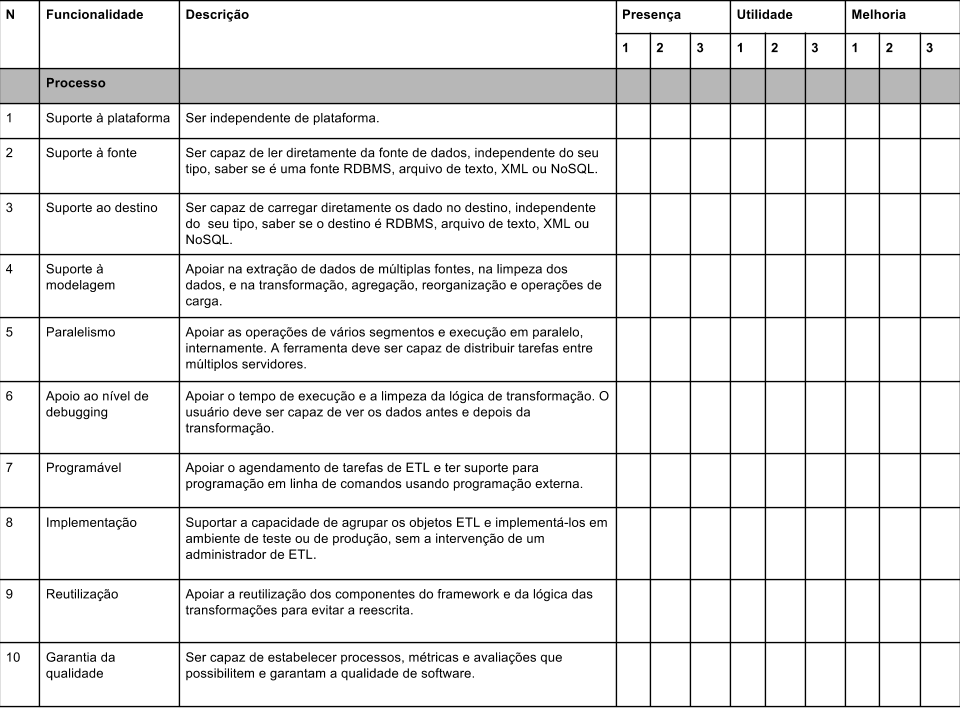
\includegraphics[scale=0.5]{fig/questionario_caracteristicas.png}
	\caption{Questionário de Funcionalidades}
	\label{questionariofuncionalidades}
\end{figure}

\clearpage

\subsection{Resultado do Estudo}


A figura \ref{presenca} apresenta o gráfico da quantidade de presença para cada funcionalidade de acordo com cada ferramenta de ETL. Já a figura \ref{utilidade} mostra o nível de importância que as ferramentas dão para cada funcionalidade e a figura \ref{melhoria} indica necessidade de melhorar funcionalidade em cada ferramenta.

\begin{figure}[h]
	\centering
	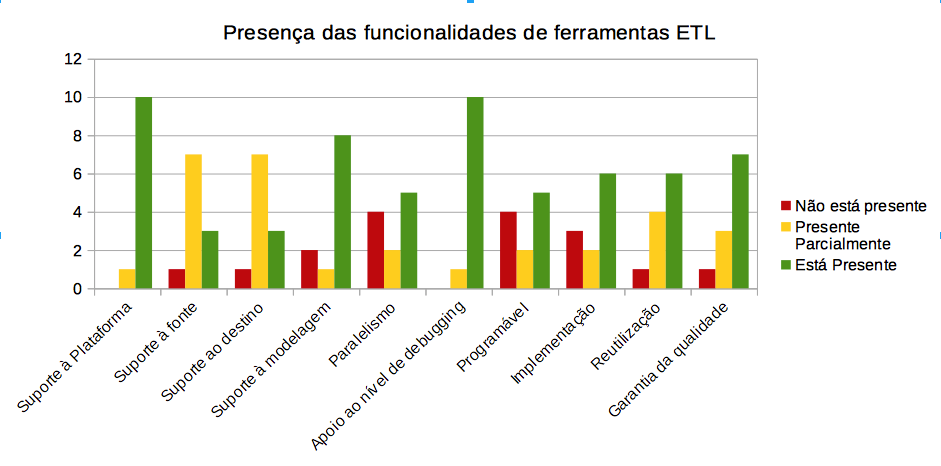
\includegraphics[scale=0.4]{fig/presenca.png}
	\caption{Quantidade de Presença para cada funcionalidade}
	\label{presenca}
\end{figure}

\begin{figure}[h]
	\centering
	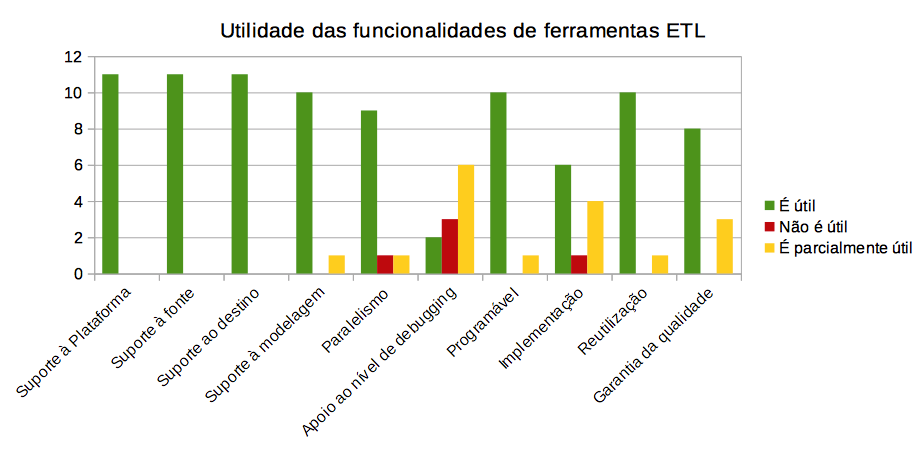
\includegraphics[scale=0.4]{fig/utilidade.png}
	\caption{Níveis de utilidade para cada funcionalidade}
	\label{utilidade}
\end{figure}

\begin{figure}[h]
	\centering
	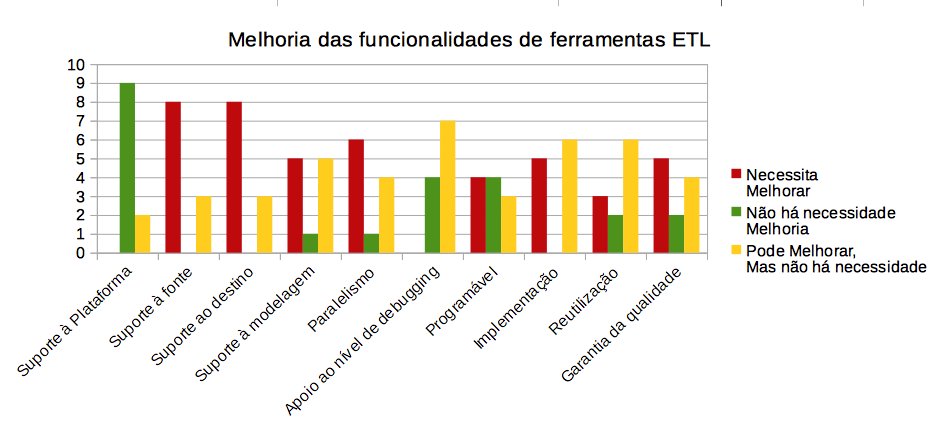
\includegraphics[scale=0.4]{fig/melhorias.png}
	\caption{Necessidade de melhoria para cada funcionalidade}
	\label{melhoria}
\end{figure}


O perfil dos participantes é apresentado no quadro \ref{resultadoperfil}, bem como a legenda para leitura é exibida no quadro \ref{legenda}. Na figura \ref{perfil} é possível comparar por meio do gráfico os perfis das ferramentas analisadas por este estudo experimental. 

Das onze ferramentas de ETL apresentadas neste estudo dez possuem código aberto, sete não possui uma marca reconhecida no mercado, nenhuma foi desenvolvida para suportar BDs NoSQL, seis possuem uma GUI, apenas quatro não são programáveis, duas não são integradas, nove delas oferece alguma alternativa para o processamento distribuído, um pouco mais da metade são extensíveis e a finalidade da maioria é modelagem tentando aliar ao desempenho.

\begin{table}[h]
	\centering
	\caption{Resultado do Perfil dos participantes}
	\label{resultadoperfil}
\resizebox{\textwidth}{!}{\begin{tabular}{|r|r|r|r|r|r|r|r|r|r|}
		\hline
		Ferramenta & Código Fonte & Marca de mercado & Para NoSQL & GUI & Programável & Integrada & Processamento & Extensível & Finalidade\\
		\hline
		PygramETL  & 1 & 2 & 2 & 2 & 1 & 1 & 2 & 1 & 2 \\
		\hline
		ARKTOSII & 1 & 2 & 2 & 1 & 2 & 1 & 3 & 2 & 1 \\
		\hline
		Big-ETL & 1 & 2 & 3 & 2 & 1 & 2 & 1 & 1 & 3\\
		\hline
		ETLMR & 1 & 2 & 2 & 2 & 1 & 1 & 1 & 1  & 2 \\
		\hline
		CloudETL & 1 & 2 & 3 & 2 & 1 & 1 & 1 & 1 & 2 \\
		\hline
		P-ETL & 1 & 2 & 3 & 1 & 2 & 1 & 3 & 2 & 3\\
		\hline
		FramETL & 1 & 2 & 2 & 2 & 1 & 1 & 2 & 1 & 1 \\
		\hline
		Talend Studio & 1 & 1 & 3 & 1 & 1 & 1 & 3 & 2 & 3 \\
		\hline
		Pentaho Kettle & 1 & 1 & 3 & 1 & 2 & 1 & 3 & 2 & 1\\
		\hline
		CloverETL & 1 & 1 & 3 & 1 & 1 & 2 & 3 & 2 & 3 \\
		\hline
		Oracle (ODI) & 2 & 1 & 3 & 1 & 2 & 1 & 3 & 2 & 3 \\
		\hline
		
		
		
	\end{tabular}}
\end{table}

\begin{table}[h!]
\centering
\caption{Legenda}
\label{legenda}
\resizebox{\textwidth}{!}{\begin{tabular}{|r|r|r|r|r|r|r|r|r|}
\hline
Código Fonte & Marca de mercado & Para NoSQL & GUI & Programável & Integrada & Processamento & Extensível & Finalidade\\
\hline
1-Aberto & 1-Reconhecido & 1-Sim & 1-Possui & 1-Sim & 1-Sim & 1-Distribuído & 1-Sim & 1-Modelagem \\
\hline
2-Fechado & 2-Não reconhecido & 2-Não & 2-Não possui & 2-Não & 2-Não & 2-Centralizado & 2-Não & 2-Desempenho \\
\hline
& & 3-Possui, mas não é o foco & & & & 3-Híbrido & & 3-Ambos \\
\hline


\end{tabular}}
\end{table}


\begin{figure}[h]
\centering
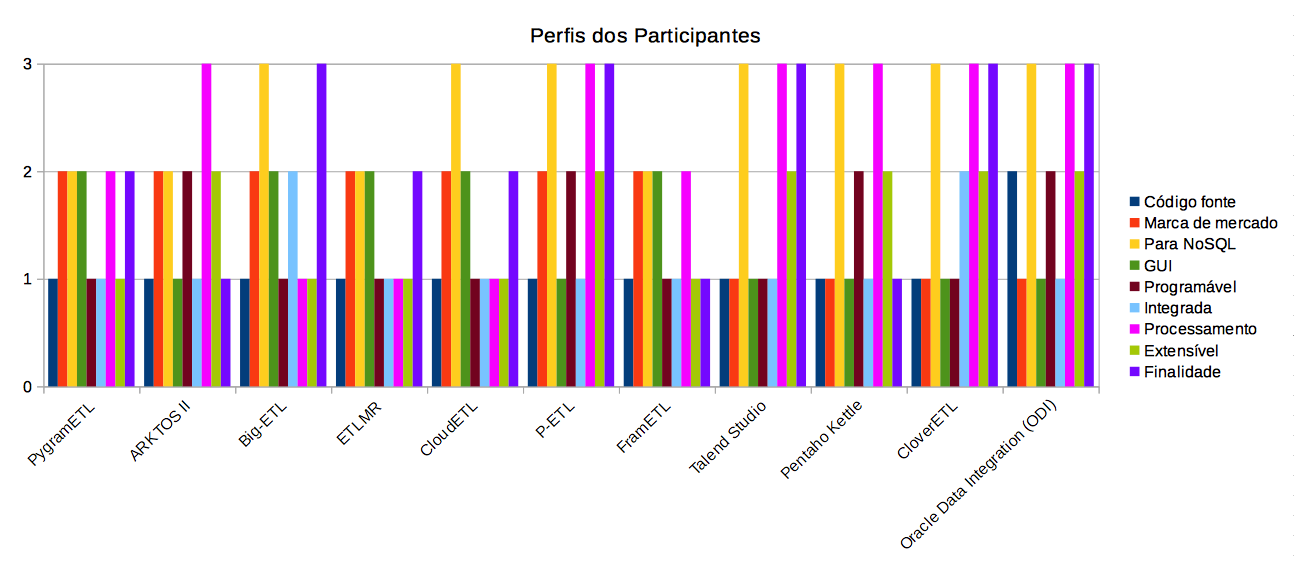
\includegraphics[scale=0.38]{fig/perfil.png}
\caption{Perfil das Ferramentas de ETL}
\label{perfil}
\end{figure}

\section{Análise e interpretação dos resultados}

Nesta seção é apresentada a análise e interpretação dos resultados conforme as regras estatísticas escolhidas para serem aplicadas neste estudo. 

\subsection{Estatística descritiva}

As medidas de tendência central como os valores "Presença", "Melhoria" e "Utilidade" são da escala ordinal, por isso é possível definir as métricas de "moda" e "mediana". As métricas de presença estão no quadro \ref{estatistica_presenca}, as métricas de utilidade são apresentadas no quadro \ref{estatistica_utilidade} e as métricas de melhoria podem ser vistas no quadro \ref{estatistica_melhoria}.

\begin{table}[h]
	\centering
	\caption{Estatística Descritiva da Presença de Funcionalidades}
	\label{estatistica_presenca}
	\begin{tabular}{|c|c|c|c|c|c|c|c|c|c|c|}
			\hline
			\multicolumn{11}{|c|}{Presença}\\
			\hline
			Funcionalidades & 1 & 2 & 3 & 4 & 5 & 6 & 7 & 8 & 9 & 10 \\
			\hline
			Mediana & 3 & 2 & 2 & 3 & 2 & 3 &2 & 3 & 3 & 3 \\
			\hline
			Moda & 3 & 2 & 2 & 3 & 3 & 3 & 3 & 3 & 3 & 3 \\
			\hline
					
			
	\end{tabular}
\end{table}

\begin{table}[h]
	\centering
	\caption{Estatística Descritiva da Melhoria de Funcionalidades}
	\label{estatistica_melhoria}
	\begin{tabular}{|c|c|c|c|c|c|c|c|c|c|c|}
			\hline
			\multicolumn{11}{|c|}{Melhoria}\\
			\hline
			Funcionalidades & 1 & 2 & 3 & 4 & 5 & 6 & 7 & 8 & 9 & 10 \\
			\hline
			Mediana & 2 & 1 & 1 & 2 & 1 & 3 & 2 & 3 & 3 & 2 \\
			\hline
			Moda & 2 & 1 & 1 & \{1,3\} & 1 & 3 & \{1,2\} & 3 & 3 & 1 \\
			\hline
			
			
	\end{tabular}
\end{table}

\begin{table}[h!]
	\centering
	\caption{Estatística Descritiva da Utilidade de Funcionalidades}
	\label{estatistica_utilidade}
	\begin{tabular}{|c|c|c|c|c|c|c|c|c|c|c|}
			\hline
			\multicolumn{11}{|c|}{Utilidade}\\
			\hline
			Funcionalidades & 1 & 2 & 3 & 4 & 5 & 6 & 7 & 8 & 9 & 10 \\
			\hline
			Mediana & 1 & 1 & 1 & 1 & 1 & 3 & 1 & 1 & 1 & 1 \\
			\hline
			Moda & 1 & 1 & 1 &1 & 1 & 3 & 1 & 1 & 1 & 1 \\
			\hline
			
			
	\end{tabular}
\end{table}

Considerando as respostas recebidas durante o estudo e utilizando os resultados de estatística descritiva podemos dividir as perguntas em 4 grupos. O primeiro grupo são as funcionalidades que estão presente, mas são parcialmente úteis; já o segundo grupo são as funcionalidades presentes e úteis; o terceiro grupo consiste na presença da funcionalidade com necessidade de melhoria; e finalmente, o quarto grupo que representa as funcionalidades que estão presentes e não necessitam de melhoria. Todos os grupos podem ser analisados nos quadros \ref{grupo1}, \ref{grupo2}, \ref{grupo3} e \ref{grupo4}.

Os valores na tabela significam P - presente:não presente; M - necessita melhoria:não necessita melhoria; U - útil;inútil. 


\begin{table}[h!]
	\centering
	\caption{Funcionalidade presente e parcialmente útil}
	\label{grupo1}
	\begin{tabular}{|c|p{4cm}|c|c|c|p{7cm}|}
	%	\hline
	%	\multicolumn{6}{|c|}{Utilidade}\\
		\hline
		N. & Funcionalidade & P & M & U & Característica  \\
		\hline
		6 & Apoio ao nível de debugging & 10:1 & 0:11 & 8:3 & - A funcionalidade existe na maioria das ferramentas, mas não dão o enfoque nela. \\
		&&&&& - É uma funcionalidade trivial, pois é possível comparar os dados da fonte e destino mesmo sem debugging.\\
		&&&&& - Pode ser útil para evitar o trabalho de fazer a comparação da fonte com o destino, além de poder dar uma resposta em tempo de execução.\\
		\hline
		
		
	\end{tabular}
\end{table}


\begin{table}[h!]
	\centering
	\caption{Funcionalidade presente e é útil}
	\label{grupo2}
	\begin{tabular}{|l|l|l|l|l|l|}
		\hline
		N & Funcionalidade & P & M & U & Características \\ \hline
		\multirow{4}{*}{2} & \multirow{4}{*}{Suporte à fonte} & \multirow{4}{*}{10:1} & \multirow{4}{*}{8:3} & \multirow{4}{*}{11:0} & \multirow{16}{*}{\begin{tabular}[c]{@{}l@{}}- As ferramentas oferecem algum suporte \\ em relação à leitura e carga da fonte e destino,  \\ porém muitas apenas lidam com RDBMS.\\ - Deve haver um enfoque nas novas soluções \\ de BDs como os BDs NoSQL.\\ - Algumas ferramentas não oferecem a opção \\ para utilizar linha de comando, o qual é \\ considerado importante para ter maior liberdade \\ na implementação de processos de ETL.\\ -Dependendo do foco da ferramenta, alguma\\ delas não dão importância ao processamento\\ em paralelo, porém em se tratando de Big Data,\\ o processamento em paralelo é fundamental\\ para possibilitar a execução de processos de\\ ETL em grandes volumes de dados.\end{tabular}} \\
		&  &  &  &  &  \\
		&  &  &  &  &  \\
		&  &  &  &  &  \\ \cline{1-5}
		\multirow{4}{*}{3} & \multirow{4}{*}{Suporte ao destino} & \multirow{4}{*}{10:1} & \multirow{4}{*}{8:3} & \multirow{4}{*}{11:0} &  \\
		&  &  &  &  &  \\
		&  &  &  &  &  \\
		&  &  &  &  &  \\ \cline{1-5}
		\multirow{4}{*}{5} & \multirow{4}{*}{Paralelismo} & \multirow{4}{*}{7:4} & \multirow{4}{*}{6:5} & \multirow{4}{*}{10:1} &  \\
		&  &  &  &  &  \\
		&  &  &  &  &  \\
		&  &  &  &  &  \\ \cline{1-5}
		\multirow{4}{*}{7} & \multirow{4}{*}{Programável} & \multirow{4}{*}{7:4} & \multirow{4}{*}{4:7} & \multirow{4}{*}{11:0} &  \\
		&  &  &  &  &  \\
		&  &  &  &  &  \\
		&  &  &  &  &  \\ \hline
	\end{tabular}
\end{table}


\begin{table}[h!]
	\centering
	\caption{Funcionalidade presente e necessita melhorar}
	\label{grupo3}
	\begin{tabular}{|l|l|l|l|l|l|}
		\hline
		N & Funcionalidade & P & M & U & Características \\ \hline
		\multirow{4}{*}{4} & \multirow{4}{*}{Suporte à modelagem} & \multirow{4}{*}{9:2} & \multirow{4}{*}{5:6} & \multirow{4}{*}{11:0} & \multirow{10}{*}{\begin{tabular}[c]{@{}l@{}}- A maioria das ferramentas dão suporte\\ à modelagem dos processos de ETL,\\ porém algumas focam apenas no \\ desempenho necessitando melhoria no \\ processo de modelagem.\\ - Poucas ferramentas dão importância \\ para garantir qualidade aos processos \\ de ETL ou ao seu desempenho.\end{tabular}} \\
		&  &  &  &  &  \\
		&  &  &  &  &  \\
		&  &  &  &  &  \\ \cline{1-5}
		\multirow{6}{*}{10} & \multirow{6}{*}{Garantia de qualidade} & \multirow{6}{*}{10:1} & \multirow{6}{*}{5:6} & \multirow{6}{*}{11:0} &  \\
		&  &  &  &  &  \\
		&  &  &  &  &  \\
		&  &  &  &  &  \\
		&  &  &  &  &  \\
		&  &  &  &  &  \\ \hline
	\end{tabular}
\end{table}

\begin{table}[h!]
	\centering
	\caption{Funcionalidade presente e não necessita melhoria}
	\label{grupo4}
	\begin{tabular}{|l|l|l|l|l|l|}
		\hline
		N & Funcionalidade & P & M & U & Características \\ \hline
		\multirow{4}{*}{1} & \multirow{4}{*}{Suporte à plataforma} & \multirow{4}{*}{11:0} & \multirow{4}{*}{2:9} & \multirow{4}{*}{11:0} & \multirow{14}{*}{\begin{tabular}[c]{@{}l@{}}- As ferramentas demonstraram ser independentes\\ de plataforma por terem características como \\ código compilável e serem programáveis. \\ - Criar processos de ETL demonstrou ser \\complexo, necessitando de algum tipo de \\experiência na área. Dessa forma, não é de \\fundamental importância que haja suporte à\\implementação para usuários não administradores.\\ - A maioria das ferramentas, por serem\\ de código aberto e programáveis, oferecem\\ a possibilidade de reutilização de código\\ ou algumas até mesmo oferecem possibilidade\\ de reusar os processos de ETL já criados.\end{tabular}} \\
		&  &  &  &  &  \\
		&  &  &  &  &  \\
		&  &  &  &  &  \\ \cline{1-5}
		\multirow{4}{*}{8} & \multirow{4}{*}{Implementação} & \multirow{4}{*}{8:3} & \multirow{4}{*}{5:6} & \multirow{4}{*}{10:1} &  \\
		&  &  &  &  &  \\
		&  &  &  &  &  \\
		&  &  &  &  &  \\ \cline{1-5}
		\multirow{6}{*}{9} & \multirow{6}{*}{Reutilização} & \multirow{6}{*}{10:1} & \multirow{6}{*}{3:8} & \multirow{6}{*}{11:0} &  \\
		&  &  &  &  &  \\
		&  &  &  &  &  \\
		&  &  &  &  &  \\
		&  &  &  &  &  \\
		&  &  &  &  &  \\ \hline
	\end{tabular}
\end{table}


\subsection{Aplicação do teste estatístico}

Para cada funcionalidade foi aplicado o teste de associação Qui-quadrado, com o objetivo de verificar se existe associação entre a ferramenta e a presença da sua funcionalidade. O teste do qui-quadrado pode ser usado em pesquisas de amostras independentes com a variável de resposta qualitativa (categórica) (\cite{barbetta:2012}). O quadro \ref{distribuicao} mostra os resultados da quantidade de funcionalidades presentes nas ferramentas do estudo.

\begin{table}
	\centering
	\caption{Quadro de resultado do valor observado de existência da funcionalidade}
	\label{distribuicao}
	\begin{tabular}{|l|l|l|l|l|l|l|l|l|l|l|l|}
		\hline
		Funcionalidade & 1 & 2 & 3 & 4 & 5 & 6 & 7 & 8 & 9 & 10 & Total \\ \hline
		Existe & 10 & 3 & 3 & 8 & 5 & 10 & 5 & 6 & 6 & 7 & 63 \\ \hline
		Não existe & 1 & 8 & 8 & 3 & 6 & 1 & 6 & 5 & 5 & 4 & 47 \\ \hline
		Total & 11 & 11 & 11 & 11 & 11 & 11 & 11 & 11 & 11 & 11 & 110 \\ \hline
	\end{tabular}
\end{table}

Dessa forma, calculamos o valor esperado para cada funcionalidade através da fórmula de frequências esperadas:
\\

E = (total da linha) x (total da coluna) / (total geral)

E = 63 x 11 / 110 = 6,3

E = 47 x 11 / 110 = 4,7
\\

Para a frequência das funcionalidades existentes o valor esperado é E = 6,3 e para frequência não existentes o valor esperado é E = 4,7.


A fórmula estatística para o teste qui-quadrado é definida por:
\\


 $ \chi^2 $ = $\sum \frac{(O-E)ˆ2}{E}$


 onde:
 a soma se estende a todas as células da tabela de contingência; 
 O representa a frequência observada na célula; e
 E representa a frequência esperada na célula.

\begin{table}
	\centering
	\caption{Quadro do resultado de $ \chi^2 $}
	\label{chiquadrado}
	\begin{tabular}{|l|l|l|l|l|l|l|l|l|l|l|}
		\hline
		Funcionalidade & 1 & 2 & 3 & 4 & 5 & 6 & 7 & 8 & 9 & 10 \\ \hline
		Existe & 2,17 & 1,72 & 1,72 & 0,45 & 0,26 & 2,17 & 0,26 & 0,014 & 0,014 & 0,077  \\ \hline
		Não existe & 2,91 & 2,31 & 2,31 & 0,61 & 0,36 & 2,91 & 0,36 & 0,02 & 0,02 & 0,1 \\ \hline
	\end{tabular}
\end{table}

Somando os valores das parcelas do  $ \chi^2 $, temos: 

$ \chi^2 $ = 20,765

com

\textit{gl} = (\textit{l} - 1) . (\textit{c} - 1) = (2 - 1) (10 - 1) = 9

Pela tabela de distribuição qui-quadrado, verificamos que a probabilidade de significância $\rho$ é inferior a 0,01. Então, para qualquer nível usual de significância ($\alpha = 0,05$), o teste detecta associação entre as funcionalidades e as ferramentas (pois, $\rho < \alpha $). Em outras palavras, o teste qui-quadrado mostrou que as ferramentas em estudo são diferentes quanto às suas funcionalidades.

\subsubsection{Análise quantitativa}

Para verificar a similaridade entre as funcionalidades existentes nas ferramentas de ETL na literatura e as funcionalidades do ETL4NoSQL é necessário calcular o valor de variável dependente.

\begin{itemize}
	\item[1.]  A mediana dos conjuntos de funcionalidades existentes nas ferramentas de ETL da literatura e as funcionalidades do ETL4NoSQL não podem ser consideradas iguais (a quantidade de funcionalidades com valor PMU \{ 1, X, X \} 7 < 10), nem diferentes (a quantidade de funcionalidades com valor PMU \{ 0, X, X \}  3 < 10). Assim, precisamos calcular o grau de similaridade segundo a fórmula do variável dependente 1:

		grau de similaridade = 7 / 10 * 100\% = 70\% 

	\item[2.] Para verificar a utilidade das funcionalidades similares, é necessário calcular o valor da variável dependente 2:

		parte útil das funcionalidades similares = 6 / 7 * 100\% =85,71\%

		parte inútil das funcionalidades similares  = 1 / 7 * 100\% = 14,29\%

	\item[3.] Para verificar a necessidade de melhoria das funcionalidades similares é necessário calcular o valor de variável dependente 3:

		parte que necessita de melhoria das funcionalidades similares = 3 / 7 * 100\% = 42,85\%

		parte que não necessita de melhoria das funcionalidades similares = 4 / 7 * 100\% = 57,15\%

\end{itemize}

\subsection{Análise qualitativa}

Para verificar as funcionalidades que não estão presentes no ETL4NoSQL neste trabalho de pesquisa, mas que são consideradas úteis para melhoria dos processos de ETL, foi feita a análise qualitativa apresentada no quadro \ref{naooferecidas}.

\begin{table}[h!]
	\centering
	\caption{Funcionalidades não oferecidas pelo ETL4NoSQL}
	\label{naooferecidas}
	\begin{tabular}{|l|l|l|l|}
		\hline
		Funcionalidade & 6 & 8 & 10 \\ \hline
		\begin{tabular}[c]{@{}l@{}}Quantidade total de ferramentas que não possuem \\ ou possuem parcialmente a funcionalidade\end{tabular} & 4 & 5 & 4 \\ \hline
		\begin{tabular}[c]{@{}l@{}}Quantidade de ferramentas que considera útil\end{tabular} & 2 & 6 & 9 \\ \hline
	\end{tabular}
\end{table}

Assim, podemos concluir que as funcionalidades 8 (implementação) e 10 (garantia de qualidade) despertam maior interesse à serem implantadas nas ferramentas de ETL. Isso pode ser explicado pelas características e aplicabilidade que as funcionalidades oferecem. As funcionalidades de implementação e garantia de qualidade, provavelmente, não estão presentes em geral ou são oferecidas de forma parcial, não sendo o foco de boa parte das ferramentas de ETL detalhadas neste trabalho. Porém, essas funcionalidades melhorariam o desempenho geral dos processos de ETL. Outras funcionalidades, não oferecidas pelas ferramentas de ETL demonstradas, e que, possivelmente são conhecidas pela literatura, mas a falta de exemplos ou aplicabilidade delas reduzem o interesse ao implementá-las.

\subsection{Verificação das hipóteses}

Para verificar o hipótese nula (H0) precisamos responder a questão Q1  (Existem funcionalidades listadas pelas ferramentas pesquisadas que não estão presentes no ETL4NoSQL?) utilizando a métrica M2. O resultado do teste Qui-quadrado mostra que 3 das 10 funcionalidades analisadas não podem ser consideradas como oferecidas pela ferramenta apresentada. Assim, podemos concluir que a lista de funcionalidades oferecidas pelas ferramentas de ETL da literatura é diferente das funcionalidades oferecidas pelo ETL4NoSQL, ou seja, "As funcionalidades oferecidas pelo ETL4NoSQL são diferentes das funcionalidades oferecidas pelas ferramentas da literatura" (hipótese alternativa H1).

Podemos dizer ainda que existe uma funcionalidade considerada pouco útil para as ferramentas de ETL analisadas (hipótese alternativa H2), pois respondendo a questão Q2 utilizando a métrica M5, o resultado do teste Qui-quadrado mostra que a funcionalidade 6 (Apoio ao nível de debugging) é considerada pouco útil para a realização de processos de ETL.

Por conseguinte, para funcionalidades presentes no ETL4NoSQL e nas ferramentas da literatura, que são úteis e necessitam melhoraria (hipótese H3), respondendo a questão Q3 com a métrica M8 o resultado de Qui-quadrado mostra que 3 funcionalidades necessitam melhoria (2, 3, 5) e outras 3 podem melhorar, mas não tem necessidade (6, 8, 9).

Finalmente, para realizar conclusões relevantes sobre a hipótese alternativa (H4) foi feita a análise qualitativa. Os resultados da análise apresentou 2 funcionalidades (8 e 10) não presentes no ETL4NoSQL e que são úteis. Assim, podemos concluir que existem funcionalidades não presentes no ETL4NoSQL, mas que são úteis e poderiam ser implementadas futuramente como melhoria para a ferramenta.

%O teste Chi-2 consiste na comparação das distribuições re resposta entre as ferramentas com a ferramenta ideal.


\section{Considerações Finais}

Este capítulo apresentou o estudo experimental de software com o objetivo principal de definir se o \textit{framework} proposto por esta pesquisa de dissertação é adequado para auxiliar no desenvolvimento de processos de ETL em dados estruturados, semi estruturados e não estruturados. Os resultados do experimento, tendo como base as ferramentas de ETL encontradas na literatura, indicaram que o \textit{framework} proposto possui uma quantidade significativa de grau de similaridade com as ferramentas encontradas na literatura, porém o estudo conclui também que existem funcionalidades úteis e não implementadas que poderiam ser melhoradas futuramente. 

No capítulo posterior esta pesquisa de dissertação é finalizada, expondo as principais contribuições, discussões sobre dificuldades e as ameaças do trabalho de pesquisa, os resultados e trabalhos futuros a partir do ETL4NoSQL.


